\section{Období jednoho měsíce - damages shrinky}

Následující část text bude věnována rozboru dat pro shrinky typu damages v období jednoho kalendářního měsíce.

\subsection{Předzpracování dat}


Vzhledem k vysokému počtu dat pro jeden kalendářní rok, 
v roce 2022 bylo v databázi evidováno přes 32 milionů záznamů o týkající se shrinků
, jsem se rozhodla provést analýzu na měsíčním výběru dat z tohoto období. Jako zkoumaný měsíc jsem vybrala měsíc říjen, neboť v porovnání s letními měsíci a Vánocemi se v říjnu nevyskytují významné sezónní výkyvy.

% [2602933,
%  2439363,
%  2756406,
%  2618723,
%  2809775,
%  2624598,
%  2462898,
%  2545123,
%  2592480,
%  2712669,
%  2543758,
%  2524416]
% 31233142

Zkoumaná říjnová data obsahují $2\ 712\ 669$ řádků a patnáct sloupců. Každý řádek odpovídá jednomu záznamu v databázi shrinku daného produktu. Sledované údaje ve sloupcích jsou: 
% \subsubsection{Sledované údaje}
\begin{itemize}
    \item ID prodejny, kategorická proměnná,
    \item ID produktu, kategorická proměnná,
    \item datum transakce, kategorická proměnná,
    \item typ shrinku, kategorická proměnná,
    \item L1, kategorická proměnná,
    \item L2, kategorická proměnná,
    \item L4, kategorická proměnná,
    \item L5, kategorická proměnná,
    \item L6, kategorická proměnná,
    \item expirace, kategorická proměnná,
    \item množství, spojitá proměnná,
    \item ztracená nákladová cena, spojitá proměnná,
    \item den v týdnu, kategorická proměnná,
    \item číslo den, kategorická proměnná,
    \item období v měsíci (rozdělení měsíce na pět částí), kategorická proměnná.
\end{itemize}
Původní sloupec datum jsem rozdělila na tři jiné proměnné, a to den v týdnu, číslo dne a období v měsíci a sloupec datum jsem vynechala. Z důvodu vysokého počtu záznamů a odlišné povahy dvou typů shrinků jsem data dále rozdělila na shrinky typu damages a shrinky typu inventory. 


% \subsection*{Damages shrinky}

\subsubsection{Výběr dat}
% výběr dle zastoupení shrinků a kategorií produktů a dle outlierů.

Nejprve jsem graficky analyzovala zastoupení shrinků v závislosti na vybraných proměnných pomocí nástroje Power BI, viz obr. \ref*{obr:rok:g:zastoupeni1}. V návaznosti na zjištěné zastoupení shrinků v datech jsem se rozhodla vybrat pouze ty typy shrinků, které tvoří více jak jedno procento z celkových nákladů (tj. náklady činily alespoň jeden milion korun). Vynechala jsem tedy shrinky s označením 5 až 9 a naopak shrinky 0 až 4 byly ponechány. Obdobně jsem přistupovala k záznamům i z hlediska kategorie produktu úrovně L1, jelikož z grafu je patrné, že majoritní zastoupení mají pouze dvě kategorie, a to kategorie superfresh a fresh produktů. Všechny záznamy se zbylými kategoriemi (HBC, others, nonfood, dry food a tobacco) jsem z datasetu odstranila. Těmito kroky jsem zredukovala původní počet řádků datasetu na $1\ 393\ 223$ řádků.

\begin{figure}[hbtp!]
    \centering
    \captionsetup{justification=centering}
    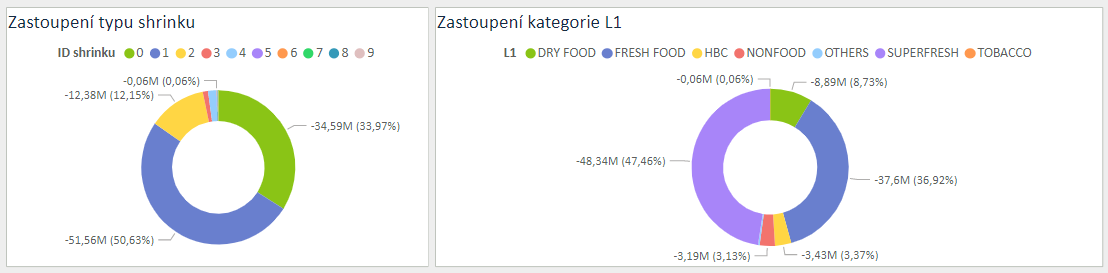
\includegraphics[width=\textwidth]{obrazky/grafy/zastoupeni1.png}
    \caption{Zastoupení shrinků typu damage a zastoupení kategorie L1 v datech \\ z října roku 2022.}
    \label{obr:rok:g:zastoupeni1}
\end{figure}

Jako cílové sloupce (\emph{target} sloupce) jsem určila sloupec s typem shrinku, množstvím produktu a nákladovou cenou. Zbylých jedenáct sloupců slouží jako vysvětlující pro-\linebreak měnné, dále budou označovány jako příznaky pro cílový sloupec. Všechny vybrané příznaky jsou kategorické proměnné, které lze dále rozdělit na nominální a ordinální. Nominální proměnné jsou ID prodejny, ID produktu, kategorie L1, L2, L4, L5 a L6. Ordinální proměnné jsou expirace, den v týdnu, číslo dne a období měsíce. Ordinální příznaky jsem přeznačila tak, aby každá obsahovala pouze hodnoty od nuly do $n_p$, kde $n_p$ je počet kategorií v $p$-tém příznaku. 

Pro další výpočty bylo vhodné přesunout se z nominálních kategorických hodnot na číselné hodnoty. Pro tyto účely jsem zvolila metodu \emph{target encoding}.  %!!! odkaz do teorie, princip meotdy je vysvětlený v kapitole...
Neboť toto kódování na numerické hodnoty zachovává velikost datového souboru, to je klíčové vzhledem k tomu, že nominální proměnné ve zkoumaných datech obsahují velký počet kategorií. Např. počet unikátních produktů v datech je $19\ 026$, což odpovídá stejnému počtu kategorií pro tuto proměnnou. Pokud bych použila one-hot kódování\footnote{One-hot kódování převádí kategorické hodnoty na numerické takovým způsobem že pro každou kategorii vytvoří samostatný sloupec s binárními hodnotami, kde 1 odpovídá dané kategorii a 0 zbylým kategoriím.}  mohlo by dojít k zásadnímu zvýšení počtu sloupců v datech, v tomto případě až o desítky tisíc. \emph{Target kódování} je podobné převodu, který jsem použila pro ordinální proměnné. Avšak na rozdíl od něj, hodnota, která je kategorii přiřazena, souvisí se zastoupením této skupiny v cílovém sloupci a nesouvisí s uspořádáním hodnot uvnitř příznaku. Nevýhodou je, že takto upravená data mohou být náchylná na overfitting, proto je potřeba při predikování použít křížovou validaci.\cite{bib:encoding}

% warehouse_id 339
% product_id 19026
% date_of_transaction 31
% motive_type 10
% cost_value 173409
% L1 7
% L2 20
% L4 141
% L5 450
% L6 1369
% expirace 330
% amount 48634
% weekday 7
% day 31
% quarter_of_month 5

Dále jsem se zabývala identifikací odlehlých hodnot. Nejprve jsem vizualizovala hodnoty pomocí grafu, obrázky \ref*{obr:rok:g:outlierN} a \ref*{obr:rok:g:outlierO}. Z grafu je patrné, že problémová je proměnná \texttt{warehouse\_id}, která označuje ID prodejny. Prodejny, které tvoří outliery mohou být malé prodejny, které kvůli menšímu počtu celkových produktů neevidují větší počet shrinků. % !!! jakeho grafu 

\begin{figure}[hbtp!]
    \centering
    \begin{minipage}{.5\textwidth}
        \centering
        \captionsetup{justification=centering}
        
        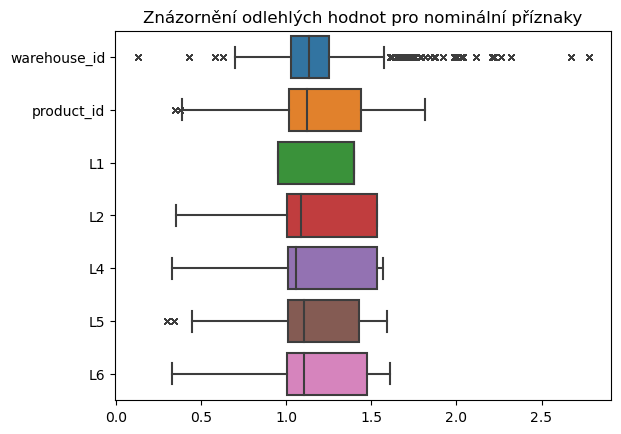
\includegraphics[width=.96\textwidth]{obrazky/zntb/box_nominal.png}
        \caption{Znázornění odlehlých hodnot pro nominální příznaky.}
        \label{obr:rok:g:outlierN}
    \end{minipage}%
    \begin{minipage}{.5\textwidth}
        \centering
        \captionsetup{justification=centering}

        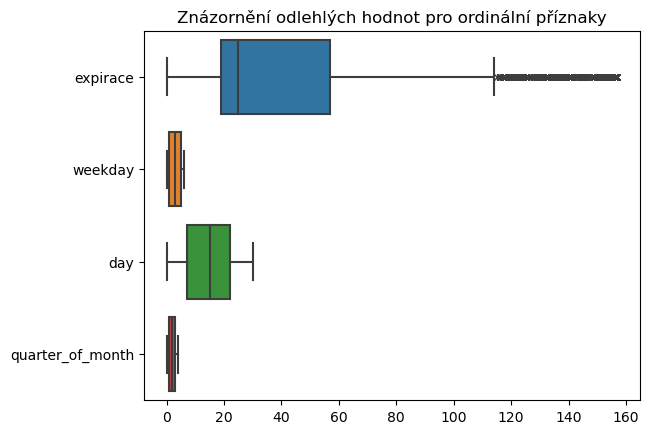
\includegraphics[width=.98\textwidth]{obrazky/zntb/box_ordinal.png}
        \caption{Znázornění odlehlých hodnot pro nominální příznaky.}
        \label{obr:rok:g:outlierO}
    \end{minipage}
\end{figure}

Pomocí Tukeyho testu jsem identifikovala přes $150\ 000$ outlierů pro příznak ID prodejny (\texttt{warehouse\_id}), čímž se dataset zredukoval na $1\ 218\ 453$ řádků. S tímto krokem klesl i počet ostatních outlierů.

V dalším kroku jsem se zaměřila na míru korelace mezi proměnnými. Vizualizovala jsem data pomocí scatter matice pro všechny proměnné, matice je možné vidět na obr. č. \ref*{obr:nb:scatter}. Z této matice můžeme na první pohled vidět, že příznaky odpovídající 4BOX kategorizaci a ID produktu vykazují závislost, což plyne z definice uspořádání této hierarchické kategorizace. V následujících krocích je cílem vybrat tu kategorii, která nejlépe popisuje data ve vztahu k shrinkům.

\begin{figure}[h!]
    \centering
    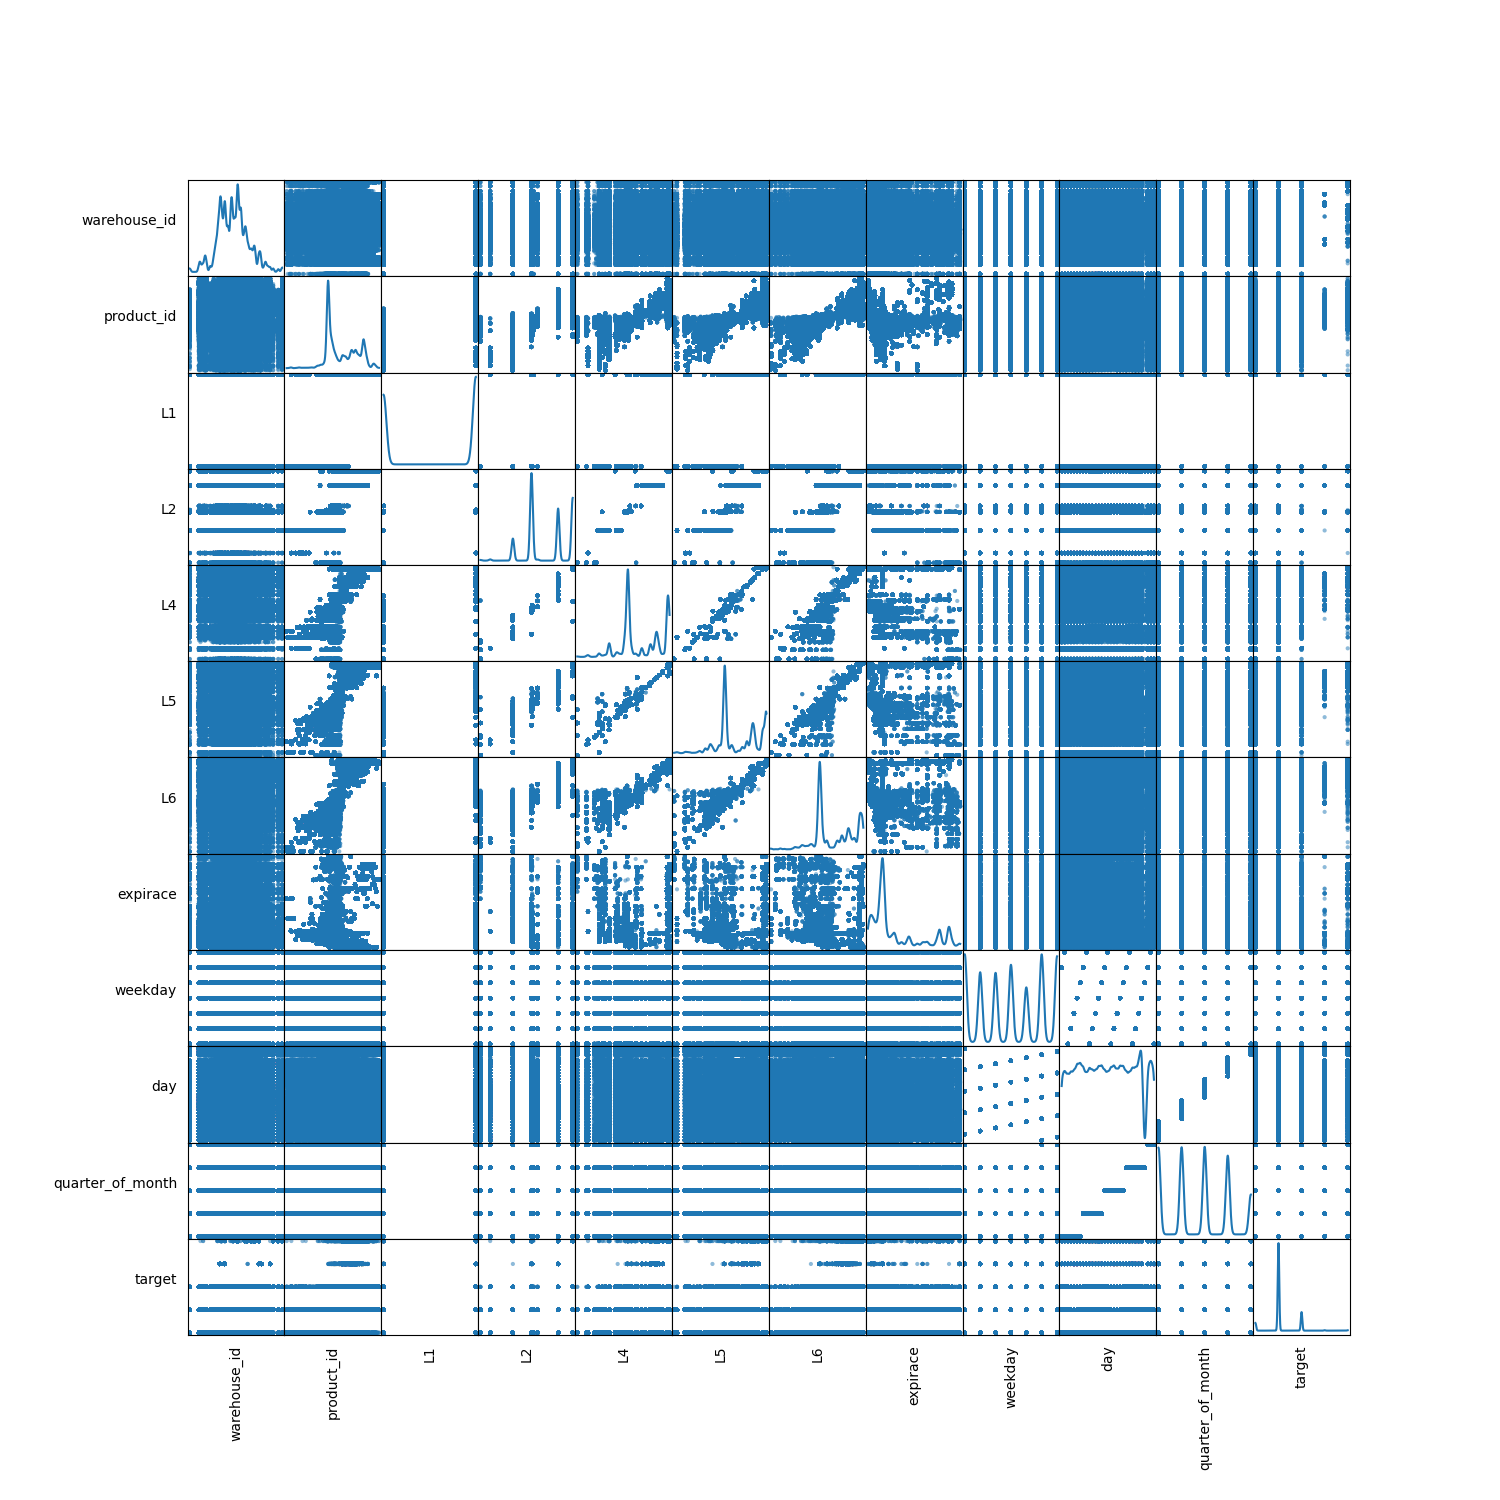
\includegraphics[width=.8\textwidth]{obrazky/zntb/MyScatter.png}
    \caption{Scatter matice příznaků.}
    \label{obr:nb:scatter}
\end{figure}
 
Jako první metodu jsem zvolila $\chi^2$ test. Vzhledem k vysokému počtu dat je matice příliš řídká, a proto nejsou výsledné hodnoty vypovídající a test je tedy pro tuto úlohu nespolehlivý.
Jiným měřítkem pro korelaci mezi proměnnými je Pearsonův korelační koeficient. %!!! odkaz na teorii
Výslednou matici popisující korelační vztahy mezi příznaky jsem vizualizovala teplotní mapou, která je zobrazena na obrázku \ref*{obr:nb:pearson}. Z výsledků je opět patrné, že mezi jednotlivými kategoriemi produktů a produkty je silná korelace. Toto zjištění je zcela logické, neboť se jedná o stromovou strukturu kategorií. Zároveň existuje korelace mezi produktovými kategoriemi a expirací produktu. p-hodnota odpovídající jednotlivým koeficientům byla vždy nulová, kromě pro koeficient týkající se dvojice proměnných expirace a ID prodejny a expirace a pořadí dne v týdnu. Je tedy možné považovat výsledky (kromě těchto dvou výjimek) za statisticky významné.

\begin{figure}[hbtp!]
    \centering
    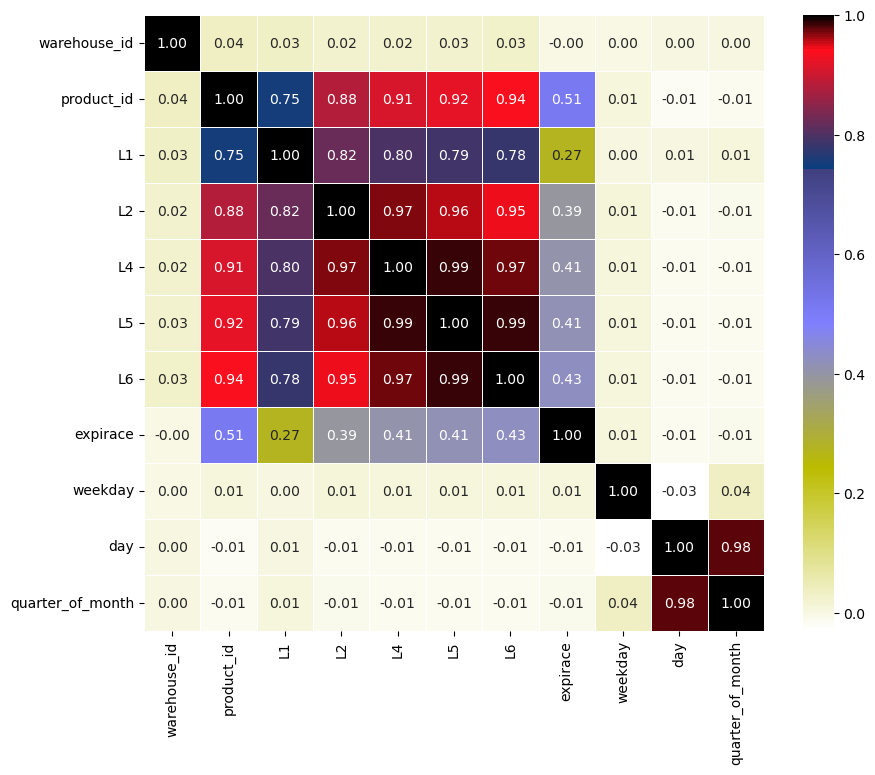
\includegraphics[width=.8\textwidth]{obrazky/zntb/pearson.png}
    \caption{Matice korelačních koeficientů mezi příznaky.}
    \label{obr:nb:pearson}
\end{figure}

Dále jsem použila výpočet koeficientů vzájemné informace\footnote{\emph{mutual information}}, který říká, jaká je podobnost mezi dvěma proměnnými \cite{bib:scikit}. % !!! odkaz na teorii
Matice vypočítaných koeficientů je na obr. \ref*{obr:nb:MI}, jelikož se jedná o symetrickou vlastnost, jsou vynechány hodnoty pod vedlejší diagonálou. Z výsledků je opět vidět, že ID produktu sdílí informaci s úrovněmi kategorizace tím více, čím je kategorizace jemnější.

\begin{figure}[hbtp!]
    \centering
    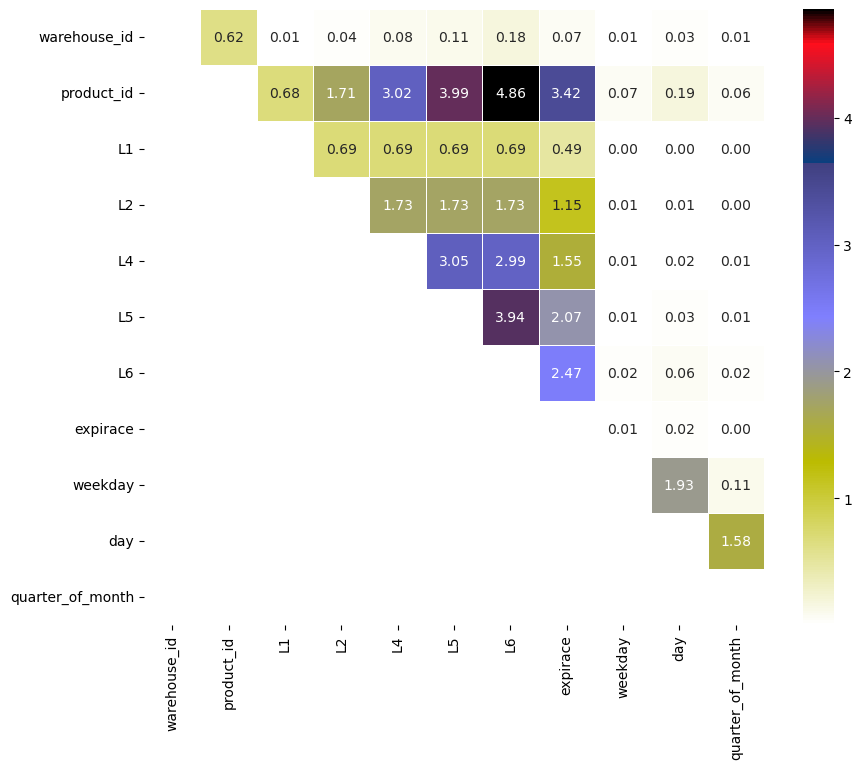
\includegraphics[width=.8\textwidth]{obrazky/zntb/MI.png}
    \caption{Matice koeficientů vzájemné informace mezi příznaky.}
    \label{obr:nb:MI}
\end{figure}

%https://www.statology.org/interpret-cramers-v/
Dále jsem pro znázornění vztahu mezi proměnnými použila koeficient Cramerovo V. Koeficient jsem postupně počítala pro každou dvojici příznaků. Koeficient nabývá hodnot mezi 0 a 1. Číslopř blízké nule indikuje, že mezi proměnnými není asociace, číslo blízké jedničce vysokou závislost \cite{bib:statology}. Na obr. \ref*{obr:nb:cramers} lze vidět, že pro kategorie L1 až L6 je hodnota koeficientu  po zaokrouhlení rovna jedné. Vysoká závislost je pak i mezi příznakem expirace a ID produktu a kategorií L1. Dále logicky mezi číslem dne a dnem v týdnu a obdobím v měsíci.
%!!! dopsat co to je %!!!zdroj, odkaz na teorii
\begin{figure}[hbtp!]
    \centering
    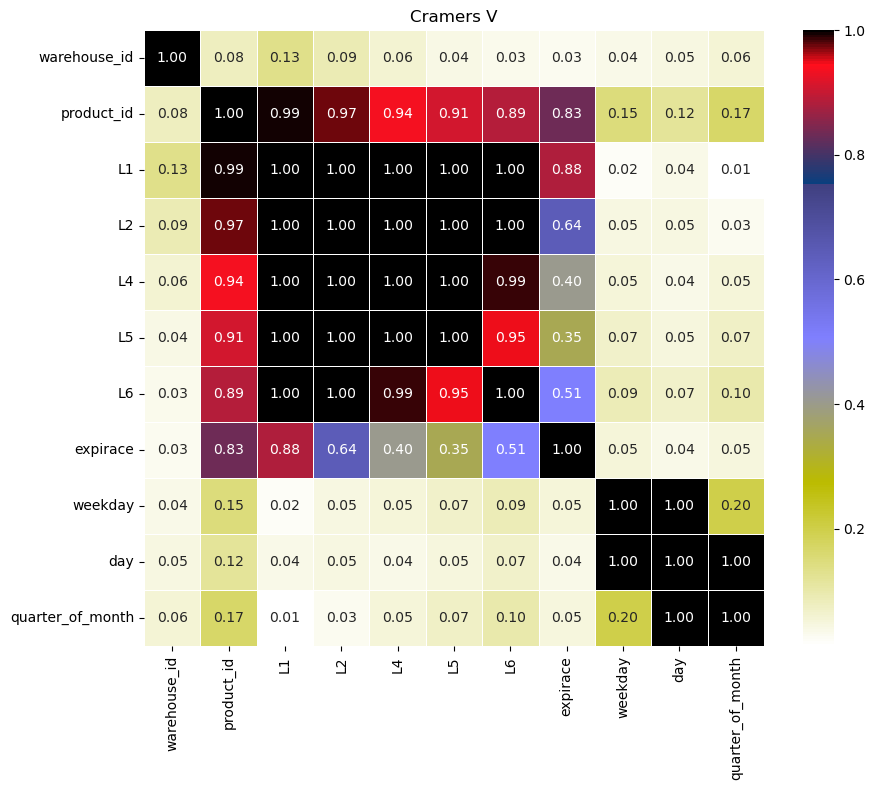
\includegraphics[width=.8\textwidth]{obrazky/zntb/cramers_u.png}
    \caption{Matice koeficientů Cramerovo V mezi příznaky.}
    \label{obr:nb:cramers}
\end{figure}

Další statistikou spočtenou na datech je Theilovo U (neboli koeficient nejistoty), který opět nabývá hodnot mezi 0 a 1 a měří vztah mezi dvěma proměnnými. Na rozdíl od předchozích statistik tento koeficient není symetrický a z výsledků lze vyvodit, ze které proměnné ze dvou zkoumaných můžeme vyvodit informaci o druhé proměnné \cite{bib:correl}. Z výsledků zobrazených v matici na obr. \ref*{obr:nb:thiels} plyne, že z ID produktu lze vyvodit část informace o kategoriích a expiraci. Zatímco úrovně L1 a L2 o ID produktu mnoho informace nenesou. Jak bylo ukázáno i v předchozích statistikách a jak vyplývá z logiky pro získání dne v týdnu a období měsíce, číslo dne nese informaci o těchto dvou příznacích.


\begin{figure}[hbtp!]
    \centering
    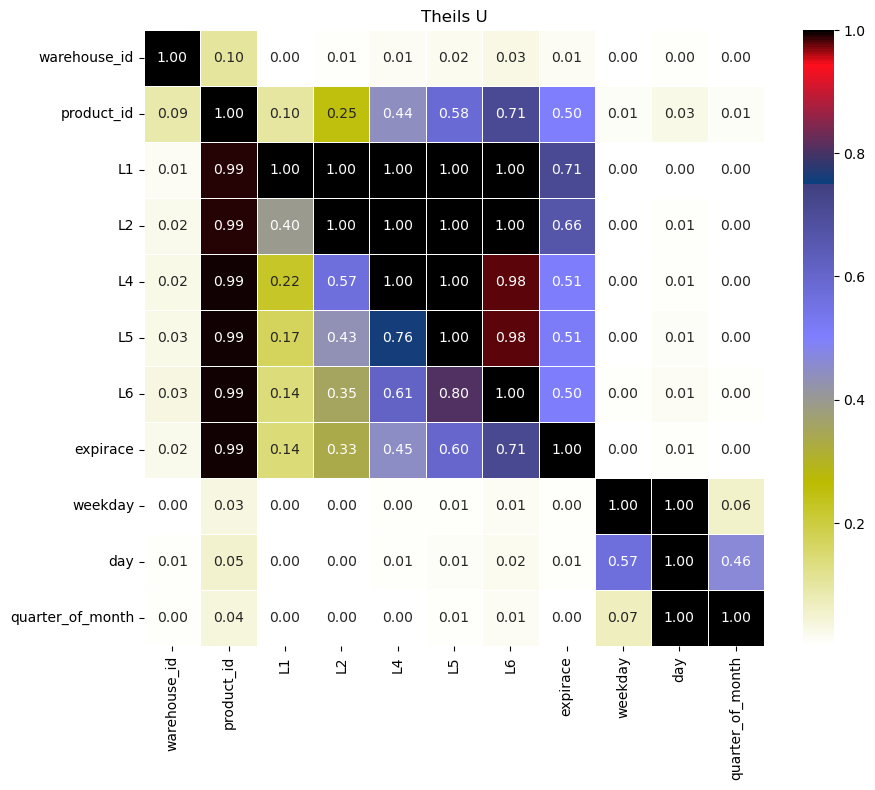
\includegraphics[width=.8\textwidth]{obrazky/zntb/theils_u.png}
    \caption{Matice koeficientů Theilovo U mezi příznaky.}
    \label{obr:nb:thiels}
\end{figure}

Z vypočítaných statistik na datasetu je patrné, že některé příznaky jsou významně závislé, a proto je třeba je z dat odstranit. Kandidáti na vynechání jsou kategorie L2, L4, L6 a číslo dne. V dalších testech budou také vybráni kandidáti a v závěru vyhodnotím, které příznaky byly podle aplikovaných metod vybrány jako vhodné k vynechání a které nikoli.

V dalším testu jsem otestovala multikolinearitu dat pomocí rozptylového inflačního faktoru (VIF). Jako hraniční faktor jsem zvolila hodnotu 40 VIF. Vysvětlující pro-\\měnné jsem odebírala z datasetu postupně a odebírání jsem ukončila až, když hodnota VIF nebyla nižší než hraniční.
Tímto došlo k redukci příznaků z jedenácti na pět, a to na kategorii L1, číslo dne, období měsíce, ID prodejny a den v týdnu. Hodnoty koeficientu VIF na datech jsou na obr. \ref*{obr:nb:vif}. 

\begin{figure}[hbtp!]
    \centering
    \begin{minipage}[t]{.5\textwidth}
      \centering
      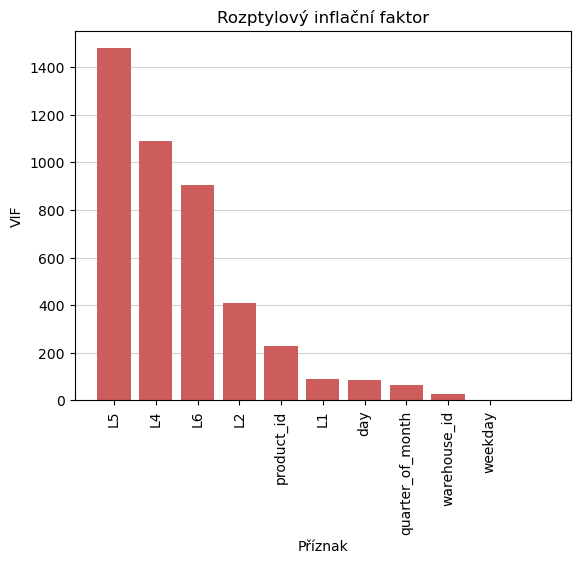
\includegraphics[width=\textwidth]{obrazky/zntb/VIF.png}
      \caption{Rozptylový inflační faktor.}
      \label{obr:nb:vif}
    \end{minipage}%
    \begin{minipage}[t]{.5\textwidth}
      \centering
      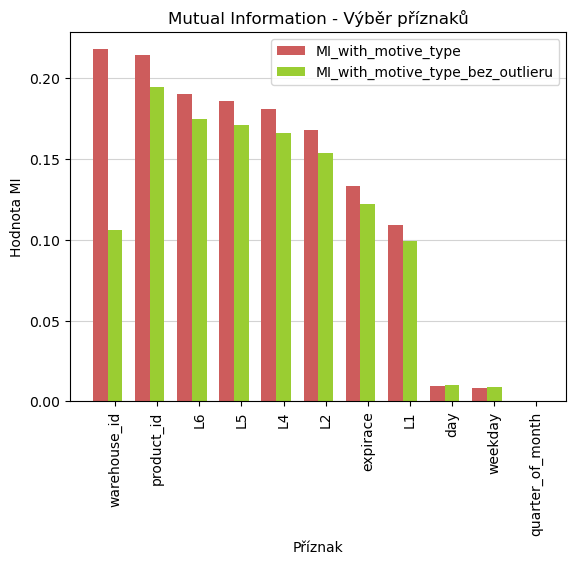
\includegraphics[width=\textwidth]{obrazky/zntb/MI_feature_selection.png}
      \caption{Koeficienty vzájemné informace mezi příznaky a cílovým sloupcem typ shrinku.}
      \label{obr:nb:MI_FS}
    \end{minipage}
    \vspace*{-1.5em}
    \end{figure}

Jako další metodu po výběr příznaků jsem vypočítala hodnotu koeficientů vzájemné informace mezi všemi příznaky s cílovým sloupcem - ID shrinku. Na obrázku \ref*{obr:nb:MI_FS} lze vidět, jak jednotlivé proměnné souvisí s cílovým sloupcem. Pro výpočet tohoto koeficientu jsem použila jak data bez outlierů, tak tenotkrát data před jejich odstraněním. Zde můžeme vidět, že významnost příznaku ID prodejny klesla o téměř polovinu. Nejvíce informace je sdíleno s ID produktu, kategorií L6, dále L5, L4, L2 a expirace. Příznaky související s časovými údaji podle tohoto kritéria nenesou mnoho společné informace.

Jako hlavní metodu pro výběr proměnných jsem se rozhodla použít metodu PCA, tuto metodu je možné použít protože kategorické proměnné jsem převedla na číselné hodnoty v předchozích krocích. Alternativou by bylo použití metody MCA, která se používá pro kategorické datasety, viz dále.
Ve své práci jsem využila implementaci PCA v knihovně \emph{Prince} v jazyce Python. 
Předtím než jsem metodu aplikovala jsem otestovala předpoklad homoskedasticity, tedy shodnost rozptylů v datech, pomocí Bartlettova testu implementovaného v knihovně \emph{factor\_analyzer}. Nulová hypotéza o shodnosti rozptylů nebyla vyvrácena (p-hodnota vyšla nulová). Metodu PCA je proto možné použít.

Na obrázcích \ref*{obr:nb:pca_roztyl_komponetn} a \ref*{obr:nb:pca_kum_roztyl_komponetn} je znázorněno prvních deset komponent a rozptyl který v datech vysvětlují. Na základě hodnot jsem vybrala prvních pět komponent. Již pátá komponenta (označená č. 4) spolu s předchozími vysvětluje více jak 95 \% variability dat. V dalším kroku jsem vypočítala příspěvky příznaků k těmto pěti komponentám a vybrala jsem ty příznaky, které přispívají nejvíce k prvním pěti komponentám. Jejich příspěvek je znázorněný na obr. \ref*{obr:nb:pca_prispevek}. Na základě výsledků analýzy hlavních komponent byly vybrány jako vhodné příznaky pro další práci s daty tyto příznaky - ++ ID prodejny, den v týdnu, expirace, den a období v měsíci.

\begin{figure}[hbtp!]
    \centering
    \begin{minipage}[t]{.5\textwidth}
      \centering
      \captionsetup{justification=centering}

      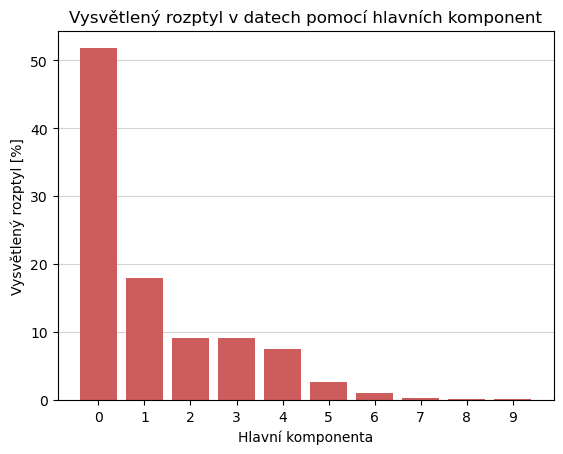
\includegraphics[width=\textwidth]{obrazky/zntb/pca-roztyl_komponetn.png}
      \caption{PCA - vysvětlený \\ rozptyl hlavních komponent.}
      \label{obr:nb:pca_roztyl_komponetn}
    \end{minipage}%
    \begin{minipage}[t]{.5\textwidth}
      \centering
      \captionsetup{justification=centering}

      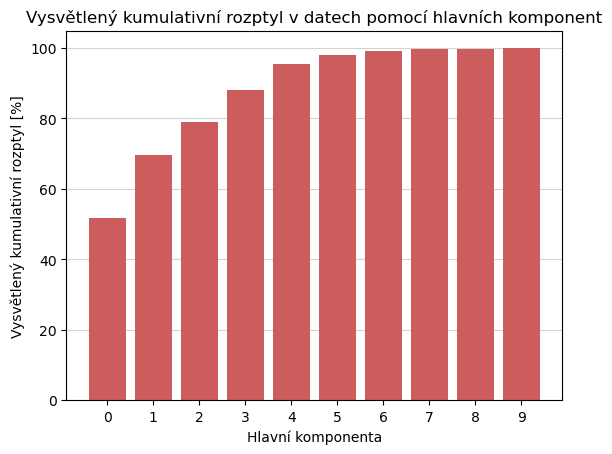
\includegraphics[width=\textwidth]{obrazky/zntb/pca-kum_roztyl_komponetn.png}
      \caption{PCA - kumulativní vysvětlený rozptyl hlavních komponent.}
      \label{obr:nb:pca_kum_roztyl_komponetn}
    \end{minipage}
    \end{figure}

\begin{figure}[h!]
    \centering
    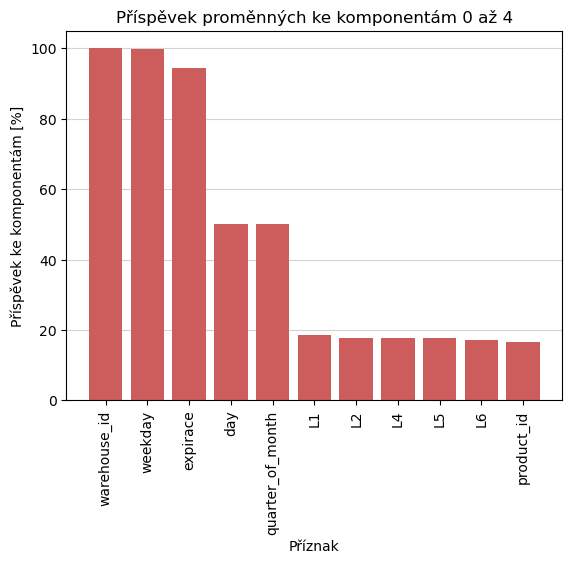
\includegraphics[width=.8\textwidth]{obrazky/zntb/pca-prispevky.png}
    \caption{Příspěvek proměnných ke komponentám 0 až 4.}
    \label{obr:nb:pca_prispevek}
\end{figure}
    
Jak již bylo zmíněno pro redukci dimenzionality u kategorických dat lze použít metodu MCA, opět jsem využila implementaci z knihovny \emph{Prince}. V této implementaci jsou nominální kategorické hodnoty kódovány tak, že narůstá počet sloupců, a proto bylo nutné, vzhledem k nárokům na paměť k uložení matice, omezit množství dat. Vybrala jsem náhodný 20\% vzorek dat, na které jsem MCA aplikovala. Vypočítala jsem prvních pět komponent, které dohromady popisují 79 \% variability dat. Jelikož byla každá kategorie chápána jako samostatná proměnná příspěvky jednotlivých příznaků ke komponentám byly rozmístěny mezi všechny kategorie, nikoli k jednotlivým příznakům. Po agregaci podle původních příznaků největší příspěvek mělo ID produktu, kategorie L6, L5, L4, zatímco nejmenší ID prodejny, L1, den v týdnu a období měsíce. Tyto výsledky je třeba brát se zvážením neboť výpočty probíhali na řádově menším vzorku než u předchozích metod.

% warehouse_id        0.024256
% product_id          1.147270
% L1                  0.035793
% L2                  0.355452
% L4                  0.841652
% L5                  0.911692
% L6                  0.930902
% expirace            0.306007
% weekday             0.035521
% day                 0.362474
% quarter_of_month    0.048981

\subsubsection*{Shrnutí pro výběr dat}

Na základě předchozích metod byly původní příznaky datasetu zredukovány na menší počet. Vzhledem k tomu, že různé metody vybraly různé příznaky, bylo stanoveno více možných výběrů.

Korelované jsou hodnoty ID produktu, L6, L5, L4 a expirace. Dále také z označení dne lze určit období měsíce. Ze zmíněných korelovaných příznaků není proto vhodné začlenit více než jeden příznak. Pokud je tato myšlenka aplikována na výsledky metod PCA a MCA a výsledků zjištěných pomocí hraniční hodnoty VIF.

\begin{enumerate}
    \item Následující sloupce byly získány podle hodnoty rozptylového inflačního faktoru. Touto metodou byl navržen i sloupec s číslem dne, ten však z důvodů korelace nebyl zahrnutý
    \begin{enumerate}
        \item[1.1.] L1, období měsíce, ID prodejny a den v týdnu.
    \end{enumerate}
    
    \item[] K této variantě existují i dvě alternativy, ve kterých je obměněna úroveň kategorizace produktu:     
    \begin{enumerate}
    \item[1.2.] L5, období měsíce, ID prodejny a den v týdnu
    \item[1.3.] L4, období měsíce, ID prodejny a den v týdnu
    \end{enumerate}
    \item Metodou PCA bylo zjištěno, které příznaky nejvíce přispívají ke komponentám, které popisují téměř 96 \% rozptylu v původních datech - jedná se o příznaky ID prodejny, den v týdnu, expirace, období v měsíci a číslo dne. Naopak metoda MCA vybrala kategorie L4 až L6 jako důležité. Sloučením a přihlédnutím ke korelačním koeficientům byly vybráno pět příznaků
    \begin{enumerate}
        \item[2.1.] ID prodejny, den v týdnu, expirace, období v měsíci, L5.
    \end{enumerate}
    \item[] Tato varianta příznaků byla ještě rozšířena o příznaky, které se týkají produktů. Přidané příznaky jsou spolu korelované, přesto 
    \begin{enumerate}
    \item[2.2.] ID prodejny, den v týdnu, expirace, období v měsíci, L5, L2
    \item[2.3.] ID prodejny, den v týdnu, expirace, období v měsíci, L5, L2, ID produktu
    \item[2.4.] ID prodejny, den v týdnu, období v měsíci, L2, ID produktu
    \item[] L2,L5, obdobi v mesici,  ID prodejny, den v týdnu, ID produktu, target
    \end{enumerate}
\end{enumerate}

Všech sedm možných výběrů bylo otestováno metodou gradient boosting. Pro další výpočty byla použita pouze varianta, která vykazovala nejlepší přesnost. Tabulka \ref*{tab:acc-gb} uvádí získané přesnosti.

\begin{table}[hbtp!]
    \centering
    \captionsetup{justification=centering}
    \caption{Tabulka dosažených přesností dosažených metodou gradient boosting pro varianty výběru příznaků.}
    \begin{tabular}{ccc}
    \multicolumn{1}{c}{\textbf{Varianta}} & \multicolumn{2}{c}{\textbf{Přesnost} {[}\%{]}} \\
    \multicolumn{1}{c}{} & \multicolumn{1}{c}{Trénovací data} & \multicolumn{1}{c}{Testovací data} \\
    \hline
    1.1. & 79{,}27                & 79{,}15\\
    1.2. & 82{,}88                & 82{,}77\\
    1.3. & 82{,}80                & 82{,}67\\
    2.1. & 83{,}21                & 83{,}07\\
    2.2. & 83{,}38                & 83{,}30\\
    2.3. & 83{,}67                & 83{,}54\\
    2.4. & 83{,}44                & 83{,}33    \\
    2.5 & 83,60&                    83,45      
    \end{tabular}
    \label{tab:acc-gb}
    \end{table}

\subsection{Klasifikace dat}

Tato část se věnuje předpovědi typu shrinku z dostupných dat. V předchozích sekcích bylo popsáno předzpracování dat a výběr vhodných příznaků pro úlohu klasifikace. Byly navrženy dvě skupiny příznaků, na kterých budou provedeny výpočty. K obě variantám se bude přistupovat stejným postupem a následně budou porovnány dosažené výsledky. 

Cílový sloupec, který je předpovídán, je pouze jeden. Jedná se o ID shrinku. To obsahuje pět různých kategorií (označené číslicemi od 0 do 4). Proto úlohu můžeme označit jako klasifikační úlohu pro více tříd (neboli \emph{multiclass classification}). Jazyk Python nabízí v knihovně \emph{scikit-learn} řadu metod, které podporují klasifikace do více tříd.\cite{bib:scikit-multiclass}

Vybrala jsem následující metody pro klasifikaci ID shrinku:
\begin{itemize}
    \item logistická regrese OVR,
    \item multinomická logistická regrese,
    \item random forest klasifikátor,
    \item gradient boosting klasifikátor.
\end{itemize} 

Logistickou regresi jsem použila jako základní metodu pro klasifikaci v případě, že vstupní dataset se skládá z kategorických proměnných \cite{bib:chooseregression}. Balíček \emph{scikit-learn} umožňuje klasifikaci do více tříd spočítat dvěma způsoby, které se liší v přístupu provedení klasifikace. 
První přístup využívá schématu OVR (\emph{One-vs-Rest} neboli jeden proti všem). Při použití OVR se každá třída trénuje samostatně. Pro každou třídu je úloha převedena na binární klasifikaci, kdy zkoumaná třída je označena jako pozitivní a všechny zbylé jako negativní. Pokud máme $N$ tříd, pak je vyhodnoceno $N$ binárních logistických regresí.
Naproti tomu multinomická log. regrese nevyhodnocuje třídy odděleně, ale používá funkci softmax. Ta predikuje zda, daný bod náleží do jedné z tříd.\cite{bib:multiregression}

Další zvolenou metodu je klasifikátor implementující random forest algoritmus. Tento algoritmus jsem zvolila vzhledem ke skutečnosti, že je úspěšně využíván pro problémy z reálného světa a dovede pracovat s velkým objemem dat, které tyto úlohy obvykle zahrnují \cite{bib:rf}. Zároveň volba parametrů pro tuto metodu je intuitivní. Poslední zvolenou metoudou je klasifkátor, který využívá gradient boosting. Tento klasifikátor také vytváří rozhodovací stromy jako random forest. Narozdíl od zmíněného klasifikátoru, jsou ale stromy vytvářeny postupně v závislosti na naposledy vytvořeném stromu. Stromy jsou k sobě agregovány během procesu trénování. Zatímco random forest vytváří stromy nezávisle a agreguje je až na konci procesu.\cite{bib:rfgb}

\subsubsection{Výsledky}

Nejprve jsem pracovala s vybranými příznaky - L1, období měsíce, ID prodejny a den v týdnu.
Data jsem rozdělila na tři skupiny - data pro trénování, validaci a testování v poměru 8:1:1. 

Naimplementovala jsem metodu \texttt{perform\_classification} umožňuje spustit vybraný model s požadovanými parametry z knihovny \emph{scikit-learn}, provede $k$-fold crossvalidaci, nafituje model na trénovací data a poté ověří přesnost na trénovacích datech. V případě, že jsou předány i parametry pro ladění, na validačních je model doladěn a pak na nejlepších parametrech opět otestován. Celá metoda se nachází v příloze této práce. % !!! doplnit do přílohy kod k funkci...

\begin{lstlisting}[language=Python, frame=none, numbers=left, numberstyle=\numberstyle, backgroundcolor=\color{backcolour}]
def perform_classification(
    model, 
    parameters, 
    train_x, train_y, valid_x, valid_y, test_x, test_y,
    tuning_parameters, 
    k-fold=5)
\end{lstlisting}

V tabulce \ref*{tab:klasifikace:VIF} jsou uvedeny přesnosti pro čtyři vybrané klasifikační metody. Uvedena je jak přesnost na trénovacích datech, tak na testovacích datech. Ve všech metodách byla použita metoda křížové validace, kdy data byla rozdělena do pěti skupin. Výsledná přesnost je pak průměrem dílčích přesností.

\begin{table}[hbtp!]
    \captionsetup{justification=centering}
    \caption{Tabulka dosažených přesností pro čtyři vybrané klasifikační metody na datech se shrinky typu damages s vybranými příznaky podle varianty 1.}
    \begin{tabular}{lcc}
        Metoda         & \multicolumn{2}{l}{Přesnost {[}\%{]}} \\
                                        & Trénovací data    & Testovací data    \\ \hline
        Logistická regrese OVR          & 77,04             & 76,95             \\
        Multinomická logistická regrese & 77,33             & 77,27             \\
        Random forest                   & 82,54             & 82,12             \\
        Gradient boosting               & 83,80             & 83,78            
        \end{tabular}
    \label{tab:klasifikace:VIF}
\end{table}


Nejlepších výsledků dosahuje klasifikátor gradient boosting. Přesnost na testovacích datech je téměř 84 \%. V obou metodách, které využívají rozhodovací stromy, jsem implementovala ladění parametrů. Na následujících obrázcích \ref{} % doplnit obrazky !!!
je znázorněna závislost mezi jednotlivými hodnotami parametrů a dosažené přesnosti.

V případě random forest klasifikátoru se jedná o parametry, které určují počet stromů, hloubku stromu, minimální počet vzorků, který má obsahovat list a minimální počet vzorků, kdy se může rozdělit uzel stromu. Pro klasifikátor gradient boosting byly také laděny parametry pro počet stromů, hloubku a dále míru učení.

Metoda random forest 

% metoda Gradient boosting classifer
% - Performing  5 -fold cross validation for  <class 'sklearn.ensemble._gb.GradientBoostingClassifier'> .

% `columns1 = ['L1', 'quarter_of_month', 'warehouse_id', 'weekday', 'target']`
% - Accuracy scores: [0.79125738 0.7928988  0.79164102 0.79304649 0.7924207 ]
% - Average accuracy score: 0.7922528784970851
% - Multinomial Logistic regression Train Accuracy ::  0.7926704159579466
% - Multinomial Logistic regression Test Accuracy ::  0.7915319337524416
%     - 30 min

% `columns2 = ['L5', 'quarter_of_month', 'warehouse_id', 'weekday', 'target']`
% - Accuracy scores: [0.82776361 0.83040015 0.82783454 0.82749087 0.82915795]
% - Average accuracy score: 0.8285294245108925
% - Multinomial Logistic regression Train Accuracy ::  0.828812571684165
% - Multinomial Logistic regression Test Accuracy ::  0.8276841258637953

% `columns3 = ['L4', 'quarter_of_month', 'warehouse_id', 'weekday', 'target']`
% - Accuracy scores: [0.82768667 0.82912292 0.82777299 0.82781916 0.82722927]
% - Average accuracy score: 0.8279262004907977
% - Multinomial Logistic regression Train Accuracy ::  0.8280780334071292
% - Multinomial Logistic regression Test Accuracy ::  0.8266910690543802

% `columns4 = ['L5', 'quarter_of_month', 'warehouse_id', 'weekday', 'expirace', 'target']`
% - Accuracy scores: [0.83163634 0.83345729 0.83200993 0.83231257 0.83187144]
% - Average accuracy score: 0.8322575145742153
% - Multinomial Logistic regression Train Accuracy ::  0.832070802924201
% - Multinomial Logistic regression Test Accuracy ::  0.8307453671027363
